%!TEX root = ../thesis.tex
% Appendix Template

\chapter{Artifacts in Optimal Extraction} % Main appendix title

\label{appendix:artifacts}


% Table of nods optimally reduced replaced by rectangular extraction and bad pixel replacement.
%!TEX root = ../thesis.tex
% Table of nods replaced for correction. 
\change{Maybe transpose \tref{tab:nod_replacement} to be shorter?}{}
\change{CHANGE \# into the ESO identification number 1b 2a etc}
\begin{table}
    \caption{Identification of all the optimally reduced nod spectra which had artefacts that were replaced by the rectangular extractions, corrected for bad pixels. The numbers represent the position in the nod cycle ABBAABBA. The number of the observation for each target is given by \#.}
    \label{tab:nod_replacement}
    \centering
    \begin{tabular}{cccccccc}
        \toprule
      & & \multicolumn{4}{c}{Detector}& \\
         Target  & \#  & 1 & 2 & 3 & 4 & Total \\ 
        \midrule
        \object{HD 4747}   & 1 & 8 & 5, 8 & 8 & 1, 5, 8 & 7\\
        \object{HD 162020} & 1 & - & 7, 8& - & - & 2\\ 
        \object{HD 162020} & 2 & - & 2 & - & 8 & 2\\ 
        \object{HD 167665} & 1 & 2, 4 & 8 & 1, 6 &  4, 5 & 7\\ 
        \object{HD 167665} & 2 & 2 & 3 & 1 & 8 & 4\\ 
        \object{HD 167665} & 3 & 6 & 3, 7 & - & 8 & 4\\ 
        \object{HD 168443} & 1& - & - & - & 7, 8 & 2\\ 
        \object{HD 168443} & 2 & - & 2, 4 & 6 & 8 & 4\\ 
        \object{HD 202206} & 1 & - & 6, 7& 1& - & 3\\ 
        \object{HD 202206} & 2 & 5 & - & 7,8 & - & 3\\ 
        \object{HD 202206} & 3 & 8 & 3 &  6 & 6 & 4\\ 
        \object{HD 211847} & 1 & - & 5, 7 & 2 & 4 & 4\\ 
        \object{HD 211847} & 2 & 2 & 1, 7 & 7 & 8 & 5\\ 
        \object{HD 30501}  & 1 & 7 & 7 & - & 8 & 3\\ 
        \object{HD 30501}  & 2 & 7, 8 & 3, 5, 7, 8 & 2, 7 & 2, 3&10 \\ 
        \object{HD 30501}  & 3 & 4, 8 & 2, 6, 7& 4, 8 & 7& 8\\ 
        \object{HD 30501}  & 4 & 1, 2, 4 & 3 & 5, 6 & 6 & 7\\
         \midrule
            &&&&&& 79/544\\
    \bottomrule
    \end{tabular} 
\end{table}

As mentioned in \sref{subsubsec:reductionartifacts} there were artifacts observed from the optimal reduction of the DRACS pipeline. In \tref{tab:nod_replacement} we provide a list of all the specific nods for each observation and detector that we observed artifacts and replaced with our explained method.  

With 8 nods per observation, and 4 detectors for the 17 observation there are 544 individual nod spectra. \tref{tab:nod_replacement} identifies 79 individual nods that contain artifacts which is 14.5\%.   Only 16/68 (23.5\%) detector observations have nods without any artifacts and no single observation has no artifacts in any nod spectra across the 4 detectors.




In this appendix we also provide more example images of the artifacts observed from the optimal reduction of the DRACS pipeline. We have selected one observation and detector for each observed target to show a variety of the artifacts observed.

In each image the top panel contains the 8 nod spectra extracted using the optimal method, including variance weighting. The middle panel contains the rectangular extraction (sum of the aperture), including the bad pixels.

It is clear that the large extracted artifacts occur due to single spikes observed in the rectangular extraction. What is unclear is why it only occurs some of the time.
 

\todo{THESE need to be properly selected and a caption given, one without any artifacts also?}
\todo{Style needs to be tweaked also}
 
 \begin{figure}
     \centering
     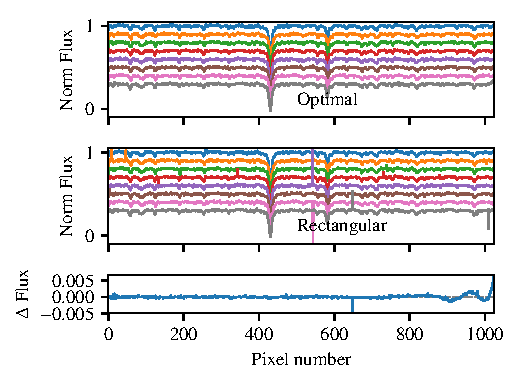
\includegraphics[width=0.7\linewidth]{figures/reduction/bp_plots/extraction_comparision_HD4747-1_chip_1}
     \caption{}
     \label{fig:extractioncomparisionhd4747-1chip1}
 \end{figure}
 \begin{figure}
     \centering
     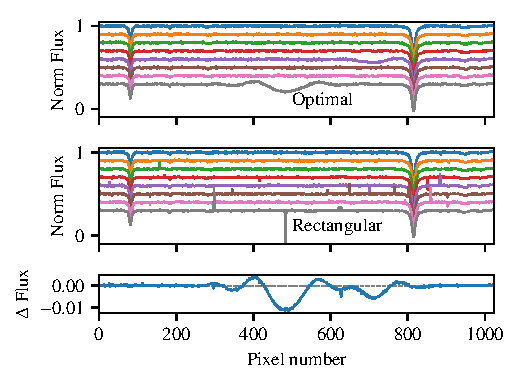
\includegraphics[width=0.7\linewidth]{figures/reduction/bp_plots/extraction_comparision_HD4747-1_chip_2}
     \caption{}
     \label{fig:extractioncomparisionhd4747-1chip2}
 \end{figure}
 \begin{figure}
     \centering
     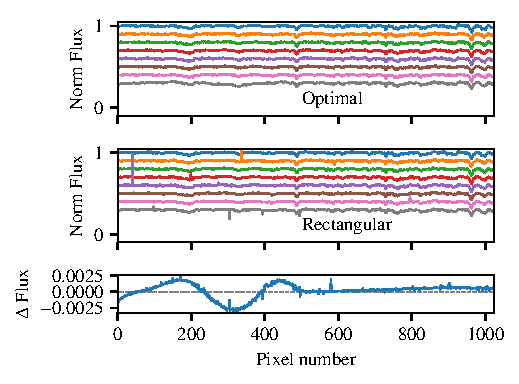
\includegraphics[width=0.7\linewidth]{figures/reduction/bp_plots/extraction_comparision_HD4747-1_chip_3}
     \caption{}
     \label{fig:extractioncomparisionhd4747-1chip3}
 \end{figure}
 \begin{figure}
     \centering
     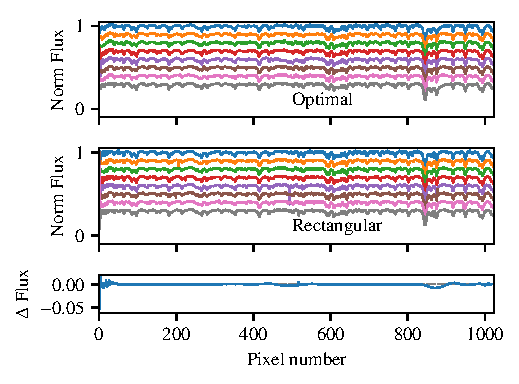
\includegraphics[width=0.7\linewidth]{figures/reduction/bp_plots/extraction_comparision_HD4747-1_chip_4}
     \caption{}
     \label{fig:extractioncomparisionhd4747-1chip4}
 \end{figure}
 \begin{figure}
     \centering
     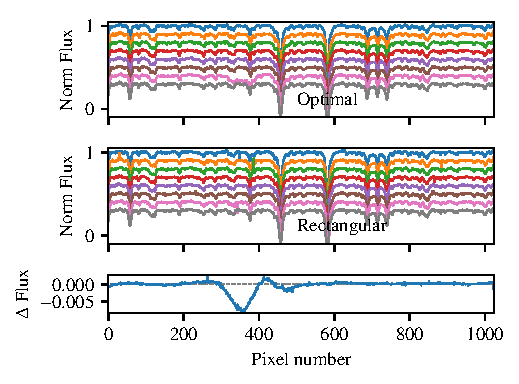
\includegraphics[width=0.7\linewidth]{figures/reduction/bp_plots/extraction_comparision_HD30501-1_chip_1}
     \caption{}
     \label{fig:extractioncomparisionhd30501-1chip1}
 \end{figure}
 